\documentclass[a4paper, oneside]{book}
\usepackage[utf8]{inputenc}
\usepackage[margin=3cm, bindingoffset=1cm]{geometry}
\linespread{1.5}
\usepackage{float}
\usepackage{csquotes}
\usepackage{subfig}
\usepackage{graphicx}
\usepackage{indentfirst}
\usepackage{fancyhdr}
\usepackage{array}
\usepackage[hidelinks]{hyperref}
\setlength{\parindent}{1cm}
\usepackage{tcolorbox}
\usepackage{multicol}
\usepackage{amssymb}

\pagestyle{fancy}
\renewcommand{\chaptermark}[1]{\markboth{\thechapter.\ \uppercase{#1}}{}}
\fancyhf{}
\fancyhead[C]{\textbf{\leftmark}}
\fancyfoot[C]{\thepage}
\renewcommand{\headrulewidth}{1pt}
\renewcommand{\footrulewidth}{1pt}
\usepackage[Conny]{fncychap}

\title{Algorithms and Protocols for Security Project}
\author{Gruppo di Fuoco}
\date{May 2024}

\renewcommand{\contentsname}{\bf Indice}
\renewcommand{\chaptername}{Capitolo}
  
\begin{document}
    %Frontespizio
    \begin{titlepage}
        \begin{center}
            \LARGE{\uppercase{Università degli Studi di Salerno}}\\
            \vspace{5mm}
            %Dipartimento
        	\uppercase{\normalsize \textbf{Dipartimento di Ingegneria dell'Informazione ed Elettrica e Matematica Applicata} }\\
        \end{center}
        
        \begin{figure}[H]
            \centering
            
\includegraphics[width=0.35\textwidth]{logo_unisa}
        \end{figure}
        
        \begin{center}
            %Corso di Laurea
        	\normalsize{ Corso di Laurea Magistrale in Ingegneria Informatica }\\
        	\vspace{15mm}
        	%Titolo
            {\LARGE{\bf \textbf{eCRED}}}\\
        	\vspace{3mm}
        \end{center}
        
        \vspace{15mm}

        \begin{center}
            \begin{tabular}{ | c | c | c | c |} \hline
                \textbf{Nome} & \textbf{Cognome} & \textbf{Matricola} & \textbf{E-Mail} \\ \hline
                    Michele & Martino & 0622702424 & m.martino48@studenti.unisa.it \\
                    \hline
                    Francesco & Quagliuolo & 0622702412 & f.quagliuolo@studenti.unisa.it \\
                    \hline
                    Emanuele & Relmi & 0622702368 & e.relmi@studenti.unisa.it \\
                    \hline
                    Benito & Senese & 0622702425 & b.senese1@studenti.unisa.it \\
                    \hline
                \end{tabular}
            \end{center}
        
        \vspace{20mm}
        
        %Anno Accademico
        \centering{\large \uppercase{Anno Accademico 2023/2024}}
    
    \end{titlepage}

    %Corpo della Tesi
    \tableofcontents
    \clearpage
    \sloppy
    \hyphenpenalty=10000
    \exhyphenpenalty=10000
    
    \chapter{WORK PACKAGE 1}
    In questo primo capitolo ci concentreremo sulla definizione degli attori onesti coinvolti nel sistema, analizzando i loro obiettivi e le funzionalità che si intendono realizzare.
    Gli attori onesti sono quegli individui o entità che agiscono in conformità con le regole e le politiche stabilite, cercando di raggiungere i loro obiettivi senza compromettere l'integrità del sistema.
    
    Successivamente, esamineremo i possibili avversari (o threat models) che potrebbero essere interessati a compromettere il sistema, esaminando le loro risorse e le motivazioni che li spingono ad agire.
    Questa analisi ci permetterà di identificare gli attacchi che il sistema potrebbe subire e di comprendere quali misure di sicurezza dovranno essere adottate per contrastarli.
    
    Una volta compreso il contesto in cui il sistema opera, identificheremo le proprietà di sicurezza che si vorrebbero preservare in presenza di attacchi.
    Queste proprietà sono fondamentali per garantire il corretto funzionamento del sistema e la protezione delle informazioni sensibili.
    
    \noindent Di seguito un elenco dettagliato di tali attori e delle loro responsabilità.

    \section{Attori del Sistema}

        \subsection{Utente}
            Gli utenti sono le persone che necessitano di accedere ai servizi qualificati offerti dai server.
            Ogni utente possiede una Carta d'Identità Elettronica (CIE), contenente un certificato digitale di tipo X.509v3, e il PIN ad essa associato.
            La CIE ha una chiave segreta di firma, utilizzabile dall'utente durante la fase di richiesta delle credenziali, garantendo così l'integrità e l'autenticità dei dati forniti alle CA.
            Il loro obiettivo è richiedere e ottenere le credenziali necessarie dalle autorità, per poi utilizzarle per accedere a servizi specifici in modo sicuro.
        
        \subsection{Server}
            I server sono entità che offrono servizi qualificati, accessibili solo ai possessori di specifiche credenziali.
            Essi devono essere in grado di verificare le credenziali presentate dagli utenti e stabilire se sono rilasciate da autorità fidate.
            Il loro obiettivo è offrire servizi in modo sicuro e limitato solo agli utenti autorizzati.
            Sono, inoltre, responsabili di gestire le richieste di accesso, garantire la sicurezza e la privacy delle operazioni e minimizzare il coinvolgimento di terze parti fidate così da ridurre i rischi legati ad un singolo punto di fallimento.
            
        \subsection{Autorità di Rilascio delle Credenziali}
            Le autorità di rilascio delle credenziali (CA) sono enti fidati che emettono credenziali agli utenti, garantendo che queste siano valide e autentiche.
            Queste autorità verificano l'identità degli utenti e le informazioni correlate prima di rilasciare le credenziali.
            Esse possono essere enti governativi, istituzioni pubbliche o altre organizzazioni autorizzate a rilasciare certificati digitali.
            Sono, quindi, responsabili di:
                \begin{itemize}
                    \item verificare e validare le informazioni degli utenti;
    
                    \item emettere credenziali autentiche;
    
                    \item garantirne la sicurezza e l'integrità;
    
                    \item mantenere un registro delle credenziali emesse.
                \end{itemize}
    
        \subsection{Autorità Rilascio CIE}
            Gli enti che si occupano dell'emissione della CIE con il PIN associato sono fondamentalmente due: l'Ufficio Anagrafe e l'Istituto Poligrafico e Zecca dello Stato (IPZS), che vengono accorpati in un'unica entità per convenienza e semplicità. Questa autorità si occupa della gestione delle pratiche amministrative relative alla registrazione delle informazioni anagrafiche e della generazione e gestione delle chiavi crittografiche e dei certificati digitali necessari per la firma elettronica. \\
            È responsabile di:
                \begin{itemize}        
                    \item produrre e consegnare la CIE, insieme al suo PIN, all'utente;
                
                    \item generare e memorizzare in modo sicuro la chiave segreta e il certificato digitale all'interno della CIE;
    
                    \item garantire che i certificati digitali siano validi e riconosciuti dalle autorità competenti;
    
                    \item implementare misure di sicurezza avanzate per proteggere la CIE da contraffazioni e accessi non autorizzati.
                \end{itemize}


    \section{Attaccanti del Sistema}
        Nel contesto del sistema descritto, è fondamentale analizzare e comprendere i potenziali attaccanti che potrebbero cercare di comprometterlo, considerando le motivazioni e le risorse a loro disposizione.
        Questi attori e gruppi di attaccanti rappresentano diverse minacce al sistema e richiedono misure di sicurezza specifiche per essere contrastati efficacemente.
    
        \begin{itemize}
            \item \textbf{Anti-Tech Theorist}
                \begin{itemize}
                    \item \textbf{Tipologia:} passivo/attivo
                    
                    \item \textbf{Descrizione:} avversario che si oppone all’innovazione e all'adozione di nuove tecnologie, sostenendo che qualunque dispositivo può essere compromesso, a discapito della privacy degli utenti.
                    Il suo scopo è quello di amplificare notizie di violazioni di dati o problemi di privacy dei sistemi per influenzare l’opinione pubblica e screditare le nuove proposte nell'ambito della sicurezza informatica.
                   
                    \item \textbf{Risorse}
                        \begin{itemize}
                            \item Abilità comunicative elevate
    
                            \item Rete di contatti con altri oppositori delle nuove tecnologie
    
                            \item Accesso ai media e ai social network per diffondere messaggi allarmistici
                        \end{itemize}
                \end{itemize}
    
            \item \textbf{The Eavesdropper}
                \begin{itemize}
                    \item \textbf{Tipologia:} passivo
                    
                    \item \textbf{Descrizione:} avversario interessato a intercettare tutte le operazioni svolte tramite il sistema (autenticazione, dati della CIE, etc.).
                    Questa tipologia di avversario può essere sia interna alle CA o ai server che esterna.
                    L'obiettivo principale è quello di collezionare le informazioni inerenti agli utenti, senza però compromettere i protocolli, i quali sono eseguiti onestamente.
                    
                    \item \textbf{Risorse}
                        \begin{itemize}
                            \item Conoscenza approfondita delle tecniche di intercettazione e analisi delle comunicazioni, nonché della crittografia utilizzata nel sistema per comprendere e interpretare correttamente i dati intercettati
    
                            \vspace{3mm}
    
                            \item Capacità di monitorare e intercettare le comunicazioni tra gli utenti e il sistema
    
                            \vspace{3mm}
    
                            \item Disponibilità di risorse computazionali significative per analizzare e elaborare grandi quantità di dati intercettati
                        \end{itemize}
                \end{itemize}
    
            \item \textbf{Malevolent Server}
                \begin{itemize}
                    \item \textbf{Tipologia:} attivo
                    
                    \item \textbf{Descrizione:} server con comportamento malevolo.
                    I suoi compiti includono: la corretta gestione delle connessioni, la verifica delle credenziali e l'erogazione del servizio richiesto.
                    Tuttavia, questa tipologia di avversario sfrutta le informazioni ricevuti dagli utenti per scopi illeciti, come il riutilizzo di informazioni personali o la vendita dei dati carpiti a terzi, compromettendo la privacy degli utenti.
                    
                    \item \textbf{Risorse}
                        \begin{itemize}
                            \item Controllo completo sui dati e sulle risorse del server, inclusi database utenti, registri di accesso e altri dati sensibili
    
                            \vspace{3mm}
    
                            \item Possibilità di accedere alle credenziali ricevute per l'accesso al servizio, consentendo di utilizzare queste informazioni per scopi illeciti.
                        \end{itemize}
                \end{itemize}
    
            \item \textbf{Identity Thief}
                \begin{itemize}
                    \item \textbf{Tipologia:} attivo
    
                    \item \textbf{Descrizione:} avversario che possiede o mira a rubare identità e/o credenziali per impersonare gli utenti legittimi e ottenere accesso non autorizzato ai servizi.
                    Potrebbe utilizzare tecniche di phishing, furto di credenziali o exploit delle vulnerabilità per ottenere informazioni sensibili e assumere l'identità di altri utenti.
    
                    \item \textbf{Risorse}
                        \begin{itemize}
                            \item Disponibilità di risorse computazionali sufficienti per eseguire attacchi brute-force, decrittazione o altri metodi per ottenere informazioni sensibili o compromettere la sicurezza del sistema
    
                            \vspace{3mm}

                            \item Possesso di un vasto database di informazioni personali ottenute illegalmente, che consente la creazione di profili dettagliati delle vittime e di utilizzare le informazioni per scopi malevoli

                            \vspace{3mm}
    
                            \item Competenze nel phishing e nell'ingegneria sociale, accesso a database di credenziali rubate, capacità di creare siti web e messaggi convincenti
                        \end{itemize}
                \end{itemize}
    
            \item \textbf{The Denier}
                \begin{itemize}
                    \item \textbf{Tipologia:} attivo
                    
                    \item \textbf{Descrizione:} avversario il cui scopo è compromettere il sistema, colpendo gli utenti o i servizi contemporaneamente.
                    Potrebbe utilizzare botnets, malware o attacchi DoS/DDoS per sovraccaricare o infiltrare il sistema, causando danni diffusi e gravi interruzioni del servizio.
                    
                    \item \textbf{Risorse}
                        \begin{itemize}
                            \item Capacità di coordinare attacchi su vasta scala
    
                            \vspace{3mm}
    
                            \item Accesso a risorse informatiche distribuite (come server cloud, dispositivi IoT compromessi o altre infrastrutture che possono essere sfruttate per eseguire questo tipo di attacchi)
    
                            \vspace{3mm}
    
                            \item Possibilità di avere motivazioni finanziarie o ideologiche significative per condurre gli attacchi, come il lucro finanziario, il furto di dati sensibili o il danneggiamento delle infrastrutture critiche per fini politici o di estorsione
                        \end{itemize}
                \end{itemize}
    
            \item \textbf{Evil Insider}
                \begin{itemize}
                    \item \textbf{Tipologia:} passivo/attivo
                    
                    \item \textbf{Descrizione:} avversario interno al sistema, che agisce in modo malevolo per ottenere benefici personali o danneggiare l'organizzazione.
                    Potrebbe rubare credenziali o informazioni sensibili, manipolare il sistema o sabotare le operazioni per raggiungere i suoi obiettivi.
                    
                    \item \textbf{Risorse}
                        \begin{itemize}
                            \item Autorizzazioni elevate all'interno del sistema, compreso l'accesso a dati sensibili e risorse critiche
    
                            \vspace{3mm}
    
                            \item Conoscenza interna dei processi e delle vulnerabilità
                        \end{itemize}
                \end{itemize}
    
            \item \textbf{The Cryptographer}
                \begin{itemize}
                    \item \textbf{Tipologia:} attivo
                    
                    \item \textbf{Descrizione:} avversario che mira a compromettere la sicurezza del sistema, attaccando le autorità di certificazione o le infrastrutture chiave del sistema di identificazione, sfruttando vulnerabilità nei protocolli crittografici utilizzati per proteggere le comunicazioni e le credenziali.
                    Potrebbe condurre attacchi di tipo man-in-the-middle, falsificare certificati o compromettere le chiavi crittografiche per ottenere accessi non autorizzati.
                    
                    \item \textbf{Risorse}
                        \begin{itemize}
                            \item Comprensione approfondita dei protocolli crittografici, dei meccanismi di autenticazione e delle vulnerabilità delle autorità di certificazione
    
                            \vspace{3mm}
    
                            \item Accesso a risorse computazionali per analizzare e rompere algoritmi crittografici
                        \end{itemize}
                \end{itemize}
    
            \item \textbf{Data Miner}
                \begin{itemize}
                    \item \textbf{Tipologia:} passivo/attivo
    
                    \item \textbf{Descrizione:} questo avversario mira a raccogliere e sfruttare i dati degli utenti per fini di analisi, profilazione o vendita a terzi
    
                    \item \textbf{Risorse}
                        \begin{itemize}
                            \item Competenze nell'analisi dei dati
                            
                            \vspace{3mm}
    
                            \item Accesso a tecnologie per l'estrazione e l'elaborazione dei dati
    
                            \vspace{3mm}
    
                            \item Comprensione delle leggi sulla privacy e delle normative sul trattamento dei dati
                        \end{itemize}
                \end{itemize}
    
            \item \textbf{The Data Harvesters}
                \begin{itemize}
                    \item \textbf{Tipologia:} attivo
    
                    \item \textbf{Descrizione:} questo gruppo mira a raccogliere e sfruttare i dati degli utenti per scopi di profitto o di spionaggio.
                    Utilizzano una combinazione di tecniche di intercettazione, furto di identità, spyware e analisi dei dati per ottenere informazioni sensibili
    
                    \item \textbf{Risorse}
                        \begin{itemize}
                            \item Competenze nell'intercettazione delle comunicazioni e nell'analisi dei dati (The Eavesdropper)
                            
                            \vspace{3mm}
    
                            \item Accesso a database di informazioni personali rubate (Identity Thief)
    
                            \vspace{3mm}
    
                            \item Capacità di elaborare grandi quantità di dati raccolti per identificare opportunità di profitto o informazioni sensibili (Data Miner)
                        \end{itemize}
                \end{itemize}
    
            \item \textbf{Crypto Conspirators}
                \begin{itemize}
                    \item \textbf{Tipologia:} attivo
    
                    \item \textbf{Descrizione:} si concentra sull'attacco alla crittografia e alla sicurezza del sistema.
                    Utilizzano competenze avanzate in crittografia, furto di identità e infiltrazione interna per compromettere la sicurezza
    
                    \item \textbf{Risorse}
                        \begin{itemize}
                            \item Competenze avanzate in crittografia e conoscenza dei protocolli di sicurezza (The Cryptographer)
                            
                            \vspace{3mm}
    
                            \item Accesso a informazioni personali rubate per ottenere accesso non autorizzato (Identity Thief)
    
                            \vspace{3mm}
    
                            \item Autorizzazioni elevate e accesso interno per facilitare gli attacchi (Evil Insider)
                        \end{itemize}
                \end{itemize}
        \end{itemize}
    
    
    \section{Proprietà}
        L'obiettivo è sviluppare un sistema che consenta l'accesso remoto a servizi riservati agli utenti in possesso delle credenziali richieste.
        In questo contesto, diverse autorità rilasciano credenziali agli utenti, i quali le utilizzano per accedere a servizi qualificati, ossia servizi limitati ai possessori di specifiche credenziali.
        
        Per garantire l'efficacia e la sicurezza del sistema, è necessario considerare diverse proprietà fondamentali: confidenzialità, integrità, trasparenza ed efficienza.
        Queste proprietà non solo assicurano che il sistema funzioni correttamente, ma proteggono anche contro potenziali minacce e abusi.
        
        \subsection{Confidenzialità}
            \begin{itemize}
                \item \textbf{C1:} I dati sensibili degli utenti devono essere protetti, ovvero accessibili solo dalle parti autorizzate in modo controllato
                
                \item \textbf{C2:} Garantire la privacy delle comunicazioni tra gli utenti e i server che offrono i servizi, in modo che non sia possibile intercettare o rubare le credenziali trasmesse
    
                \item \textbf{C3:} Garantire la privacy delle comunicazioni tra gli utenti e le autorità di rilascio delle credenziali, in modo che non sia possibile carpire dati personali relativi agli utenti
                
                \item \textbf{C4:} Tutelare gli utenti contro i malintenzionati, di modo che questi ultimi non possano utilizzare l'identità di altri utenti, firmando certificati falsi o accedendo ai servizi sfruttando le loro credenziali
            \end{itemize}
    
        \subsection{Integrità}
            \begin{itemize}
                    \item \textbf{I1:} Preservare l'integrità delle credenziali rilasciate, garantendo che non possano essere alterate o falsificate
                
                \item \textbf{I2:} I server devono garantire che le credenziali esibite dagli utenti siano verificabili e autentiche, ovvero rilasciate da autorità riconosciute come affidabili
    
                \item \textbf{I3:} Verificare che la CIE sia riconducibile all'utente che la utilizza
                
                \item \textbf{I4:} Se un servizio è rivolto ad un individuo in possesso di due credenziali allora non deve essere possibile per due utenti, ciascuno avente una sola credenziale, combinare le loro informazioni per accedere al servizio
            \end{itemize}
    
        \subsection{Trasparenza}
            \begin{itemize}
                \item \textbf{T1:} Il sistema di autenticazione dovrebbe basarsi su algoritmi noti e verificabili, di modo da permettere una verifica di essi da parte degli utenti, rendendo arduo il processo di manomissione da parte di un malintenzionato, senza che quest'ultimo sia scoperto
            
                \item \textbf{T2:} Il processo di rilascio delle credenziali deve essere trasparente e verificabile da tutte le parti coinvolte, riducendo la dipendenza da terze parti fidate così da ridurre il rischio di abuso   
                
                \item \textbf{T3:} Assicurarsi che le politiche di accesso ai servizi siano chiare e comprensibili, consentendo agli utenti di sapere quali credenziali siano necessarie per accedere agli stessi, limitando così la possibilità di accessi non autorizzati
    
                \item \textbf{T4:} La fiducia in specifiche parti deve essere giustificata da motivazioni concrete, come la possibilità di rilevare e punire abusi o il preservare la buona reputazione
            \end{itemize}
    
        \subsection{Efficienza}
            \begin{itemize}
                \item \textbf{E1:} Il sistema deve consentire ai server di controllare l'accesso utilizzando politiche avanzate e flessibili, permettendo di definire criteri di accesso complessi e specifici
                
                \item \textbf{E2:} Garantire che il processo di rilascio e verifica delle credenziali sia eseguito in modo rapido ed efficiente, riducendo al minimo i tempi di attesa e l'impatto sulle prestazioni del sistema
                
                \item \textbf{E3:} Assicurare che l'ottenimento delle credenziali tramite CIE avvenga in modo semplice e veloce, facilitando l'accesso remoto ai servizi digitali
    
                \item \textbf{E4:} Progettare il sistema in modo che possa gestire un grande numero di utenti e richieste contemporaneamente senza degradare le performance
            \end{itemize}
    
    
    \section{Completeness}
        In questo paragrafo verrà definita la completeness, la quale illustra il comportamento del sistema nel caso in cui tutte le parti coinvolte si comportino onestamente.
        
        \noindent Nello specifico:

        \begin{itemize}
            \item l'utente possessore della CIE richiede le credenziali necessarie alle autorità di rilascio

            \item le CA verificano la firma della CIE e l'identità dell'utente e, in caso positivo, emettono le credenziali 

            \item l'utente detentore delle credenziali può quindi richiedere l'accesso ad un servizio specifico, istanziato su un server

            \item il server sottopone l'utente ad un'autenticazione prima di permettere l'accesso al servizio

            \item l'utente onesto accede al servizio
        \end{itemize}
    \chapter{WORK PACKAGE 2}
    In questo capitolo verrà posta attenzione sul presentare una soluzione che risponde al modello identificato nel \textit{Work Package 1 (WP1)}.
    L’obiettivo è di proporre un sistema che riesca a raggiungere un ragionevole compromesso tra efficienza, trasparenza, confidenzialità e integrità.

    \noindent Concentreremo la nostra attenzione sui seguenti problemi chiave:
    
    \begin{itemize}        
        \item Richiesta e ottenimento, dalle CA, delle credenziali necessarie per l'accesso ai servizi specifici
        
        \item Autenticazione e accesso ai servizi qualificati
    
        \item Protezione della privacy e dell'integrità delle credenziali
    \end{itemize}


    \section{Panoramica Generale di Funzionamento}
        Innanzitutto ogni utente possiede una CIE, con al suo interno un certificato X.509v3, ed il PIN ad essa associato.
        Ciascuno di essi, tramite l'utilizzo della CIE, può richiedere delle credenziali ad un'autorità di rilascio delle stesse.
        Esistono varie autorità che rilasciano credenziali agli utenti e, una volta entratone in possesso, è possibile utilizzarle per identificarsi e accedere ai servizi qualificati.
        È consentito, all’utente, l'accesso ai servizi qualificati solo se le credenziali soddisfano i requisiti di accesso imposti dal servizio stesso.


    \section{Generazione e Utilizzo delle Credenziali}
        In questa sezione verrà sviluppato un protocollo per la generazione e l'utilizzo di un sistema di identificazione tramite credenziali per l'accesso a servizi digitali qualificati.
        Questo processo coinvolge i seguenti attori chiave: l'utente, l'autorità di rilascio delle credenziali e il server del servizio.
        Gli utenti interagiscono con la CA per la richiesta e l'ottenimento delle credenziali, e con il server per usufruire dei servizi offerti.
        Si inizierà descrivendo come un utente può richiedere una credenziale all'autorità, chiarendone anche il processo di rilascio.
        Successivamente, verrà delineato il contenuto e la struttura delle credenziali, affinché possano essere utilizzate come strumento digitale per l'identificazione e l'accesso ai servizi, mantenendo un'alta riservatezza delle informazioni contenute.
        Infine, analizzeremo il processo di identificazione e accesso a un servizio digitale.
                
        \subsection{Supposizioni}
            Il funzionamento del protocollo proposto si basa sulle seguenti supposizioni:

            \begin{itemize}
                \item Le istituzioni che si occupano dell'emissione della CIE, con annesso il suo PIN, sono assunte come parte fidata
            
                \item Ogni utente dispone inizialmente della propria CIE e del PIN associato

                \item Il certificato digitale presente nella CIE è di tipo X509v3
                
                \item All'interno del certificato sono presenti i dati che sono leggibili su una carta di identità

                \item Le autorità di rilascio sono fidate ed emettono credenziali corrette

                \item Gli algoritmi e i protocolli utilizzati sono pubblici, così da avere maggiore trasparenza e dare modo agli utenti di verificarne gli aspetti critici
            \end{itemize}

            \noindent Si procede adesso con l’analisi dettagliata di quanto delineato fino a questo momento.

        \subsection{Processo di Richiesta e Rilascio delle Credenziali}
            
            \subsubsection{Generazione di una coppia di chiavi}
                \begin{itemize}
                    \item Ogni utente genera una coppia di chiavi pubblica/privata
    
                    \item La chiave pubblica $pk_{utente}$ è generata in accordo all'algoritmo Gen(1$^n$)
                \end{itemize}
            
            \subsubsection{Richiesta ed Emissione delle Credenziali}
                \begin{itemize}
                    \item Le comunicazioni tra le CA e gli utenti avvengono tramite canali cifrati con TLS 

                    \item  L'utente invia il certificato X.509v3 relativo alla sua CIE alla CA, insieme alla richiesta della specifica credenziale

                    \item La CA invia una \textit{challenge} $b$ di bit casuali inviandola all'utente

                    \item L'utente inserisce il PIN della sua CIE e calcola l'hash $h = H(b)$ dei bit ricevuti \\
                    \textbf{NOTA:} $H : \{ {0, 1 \} }^n \rightarrow \{ {0, 1\} }^{256}$ è una funzione hash di tipo SHA-256, con dominio illimitato e codominio di dimensioni pari a 256 bit

                    \item Viene inviata una query $Sign_{sk_{CIE}}(PIN, b)$ alla CIE

                    \item La CIE verifica il PIN e, se corretto, rilascia una firma $\sigma_{CIE}$ ECDSA del messaggio (la \textit{challenge}) $b$.

                    \item L'utente, infine, invia la firma $\sigma_{CIE}$ all'autorità 
                    
                    \item La CA verifica l'identità dell'utente e, se valida, emette una credenziale firmata digitalmente, sotto forma di certificato X.509v3, contenente le informazioni specifiche richieste dal soggetto
                \end{itemize}
    
        \subsection{Processo di Identificazione e Accesso ai Servizi}
            Quando un utente presenta una credenziale per accedere a un servizio, il servizio deve verificare che l'utente possieda effettivamente la chiave privata utilizzata per firmare il documento X.509, corrispondente alla chiave pubblica inclusa nello stesso.
            Anche in questo caso, le comunicazioni tra utenti e server sono protette da canali cifrati tramite TLS.
    
            \subsubsection{Autenticazione dell'Utente}
                Quando l'utente desidera accedere a un servizio, utilizza lo schema di firma di Schnorr per autenticarsi al server.
                Nello specifico, l'utente rappresenta il \textit{prover $P$}, mentre il server il \textit{verifier $V$}.
                In questo modo, l'utente dovrà dimostrare al server di essere a conoscenza del segreto (la $sk_{utente}$, indicata con $x$) a partire dalla $pk_{utente}$ (indicata con $y = g^x$).
                
                \noindent Il protocollo si articola come segue:

                \begin{itemize}
                    \item l'utente seleziona un valore casuale $r \in \mathbb{Z}_q$, calcola $a = g^r$ e invia quest'ultimo al server

                    \item il server sceglie una stringa casuale $c \in \mathbb{Z}_q$ e lo invia all'utente

                    \item l'utente invia al server il valore $z = r + cx$, con $z \in \mathbb{Z}_q$
                \end{itemize}

                \noindent Il server, poiché $g^z = a y^c$, riesce a capire che, a richiedere il servizio, è la persona realmente in possesso delle credenziali.
    
            \subsubsection{Verifica delle Credenziali}
                \begin{itemize}
                    \item Il servizio riceve, dall'utente, la credenziale tramite certificato X.509 e ne verifica la firma digitale

                    \item Verifica, inoltre, che il numero di serie della credenziale non sia incluso nell'elenco delle revocazioni più aggiornato (CRL)
    
                    \item Controlla che le informazioni contenute nella credenziale soddisfino i requisiti di accesso
                \end{itemize}
    
            \subsubsection{Accesso ai Servizi}
                \begin{itemize}
                    \item Per garantire un accesso sicuro e affidabile ai servizi, è stata implementata una strategia anti-spam basata su puzzle parametrizzati, la quale funge da PoW (Proof of Work)
                    
                    \item Durante il processo di accesso, il server genera un puzzle matematico complesso che richiede l'elaborazione da parte dell'utente per essere risolto. La corretta risoluzione del puzzle costituisce quindi un requisito fondamentale per l'accesso ai servizi qualificati.

                    \item Superato il puzzle parametrico, il client procede con l'autenticazione basata su Schnorr

                    \item Una volta fatto ciò, il server verifica la firma dell'emittente del certificato e se le credenziali sono ancora valide
                    
                    \item Se le credenziali soddisfano i requisiti di accesso imposti dal servizio e non sono state revocate, l'utente ottiene l'accesso al servizio richiesto
                    
                    \item Il server registra l'accesso dell'utente in modo sicuro e trasparente, mantenendo un log degli accessi per future verifiche
                \end{itemize}


        \subsection{Configurazione certificati X.509v3}
            I certificati adottano la struttura standard, la quale prevede:
            \begin{multicols}{2}
                \begin{itemize}
                    \item la specifica della versione;
                        
                    \item il numero seriale;
    
                    \item il tipo di algoritmo di firma e i suoi parametri;
    
                    \item la CA che ha emesso il certificato;
    
                    \item il periodo di validità, indicato da una data d'inizio e una di fine;
    
                    \item il richiedente;
    
                    \item informazioni sulla chiave pubblica del richiedente, ovvero l'algoritmo utilizzato e la chiave pubblica stessa;
    
                    \item ID univoco dell'autorità
                        
                    \item ID univoco soggetto
                \end{itemize}
            \end{multicols}
                
            \subsubsection{Certificato digitale interno alla CIE}
                Per questo tipo di certificato sono presenti anche le seguenti estensioni:
                
                \begin{itemize}
                    \item Key Usage: Digital Signature
                    
                    \item Extended Key Usage: Client Authentication
                \end{itemize}

                \noindent Inoltre, anche i dati anagrafici, presenti sulla CIE, sono incorporati nel documento:

                \begin{multicols}{2}
                    \begin{itemize}
                        \item Comune o Ufficio Consolare emettitore
                        
                        \item Nome
                        
                        \item Cognome
                        
                        \item Luogo di nascita
                        
                        \item Data di nascita
                        
                        \item Sesso
                        
                        \item Statura
                        
                        \item Cittadinanza
                        
                        \item Codice fiscale
                        
                        \item Indirizzo di residenza
                    \end{itemize}
                \end{multicols}

            \subsubsection{Certificato digitale per le credenziali}
                In questo X.509v3, sono presenti le seguenti estensioni:
                
                \begin{itemize}
                    \item Custom Extension: Credenziale Richiesta dall'Utente
                    
                    \item CRL Distribution Point: URL della lista di revoca dei certificati (CRL)
                \end{itemize}
                
        
        \subsection{Politiche di Revoca e Aggiornamento della Certificate Revocation List (CRL)}
            \begin{itemize}
                \item Ogni certificato X.509 emesso contiene un numero di serie univoco
    
                \item Se un utente sospetta che la sua chiave privata sia stata compromessa o persa, può richiedere alla CA la revoca del certificato corrispondente
    
                \item La CA mantiene un database dei numeri di serie dei certificati emessi e revocati
    
                \item Periodicamente, la CA genera una Certificate Revocation List (CRL) contenente i numeri di serie dei certificati revocati e la firma digitale della CA
    
                \item La CRL include anche un campo CRL Distribution Point che indica l'URL da cui è possibile ottenere l'ultima versione della CRL
    
                \item I server dei servizi verificano la validità delle credenziali confrontando il numero di serie della credenziale con la CRL più aggiornata
            \end{itemize}

        \subsection{PoW: Puzzle Parametrizzato}
            Quando l'utente cerca di connettersi al server erogatore di un servizio, deve innanzitutto risolvere un puzzle parametrizzato.
            Per la sua costruzione si è scelto SHA-256, ottenendo $Z$, un sottoinsieme del codominio della CRHF, composto quindi da stringhe di 256 bit.
            L’obiettivo è quello di chiedere all'utente di trovare un valore $x$ tale che $H(rand||x) \in \mathbb{Z}$.
            

    \section{Specifiche degli algoritmi utilizzati}
        \subsection{Gen}
            L’algoritmo $Gen(1^n)$ è utilizzato per generare la coppia di chiavi pubblica e privata.
            Tramite questo algoritmo si va ad istanziare il problema del logaritmo discreto ($DLog$) ottenendo $\mathbb{G}_q$, $q$, $g$ come informazioni, dove:

            \begin{itemize}
                \item $\mathbb{G}_q$ è un gruppo ciclico di ordine primo $q$

                \item $q$ è il numero di elementi presenti nel gruppo

                \item $g$ è un generatore del gruppo
            \end{itemize}

            \noindent A questo punto, è possibile selezionare un certo valore $x \in \mathbb{Z}_q$ e calcolare $y = g^x \bmod{q}$.
            
            \noindent La chiave pubblica, indicata con $pk$, è:
            $$\langle G_q, q, g, y \rangle$$
            
            \noindent La chiave privata, indicata con $sk$, è:
            $$\langle G_q, q, g, x \rangle$$

        \subsection{Sign$_{sk}$}
            $Sign_{sk}(m)$ è un algoritmo di firma digitale, in particolare, si fa riferimento allo schema di firma di Schnorr.
            Quest'ultimo, prendendo in input un messaggio $m$ ed una chiave privata $sk$, restituisce una coppia $(z, a)$, rappresentante la firma indicata generalmente con $\sigma$, dove:

            \begin{itemize}
                \item $a$ rappresenta un contributo casuale del gruppo, tale che $a = g^r \bmod{q}$, con $r \in \mathbb{Z}_q$

                \item $z = r + H(y||a||m) x$, dove $H(\cdot)$ è un \textit{random oracle}, implementato con SHA-256
            \end{itemize}

        \subsection{Verify$_{pk}$}
            La funzione $Vrfy_{pk}(m, \sigma) : {0, 1}$, prendendo in input una chiave pubblica $pk$, un messaggio $m$ e una firma $\sigma = (z, a)$, verifica che $\sigma$ sia una firma valida per $m$, ciò avviene verificando che $g^z \equiv ay^c \bmod{q}$.

    
    \section{Protezione della Privacy e Integrità delle Credenziali}
        Per proteggere la privacy degli utenti e l'integrità delle credenziali:
        \begin{itemize}
            \item L'utilizzo di firme digitali e connessioni TLS garantisce la sicurezza e l'integrità delle comunicazioni
            
            \item Le credenziali sono emesse come documenti X.509 e contengono solo le informazioni strettamente necessarie per l'accesso ai servizi, riducendo l'esposizione di dati personali
                
             \item L'identità dell'utente non è rivelata al server del servizio qualificato attraverso i documenti X.509 delle credenziali, a meno che non sia strettamente necessario
                
             \item Le credenziali sono firmate digitalmente dalle autorità di rilascio, garantendo che non possano essere alterate o falsificate
        \end{itemize}
    
    
    \section{Conclusione}
        La soluzione proposta mira a raggiungere un compromesso tra efficienza, trasparenza, confidenzialità e sicurezza.
        Il sistema descrive dettagliatamente le azioni delle parti oneste coinvolte, garantendo che le credenziali siano emesse e verificate in modo sicuro e trasparente.
        L'uso di certificati X.509 firmati digitalmente dalle autorità di certificazione (CA) assicura che le credenziali siano autentiche e non alterabili.
        Inoltre, l'adozione del protocollo TLS per le comunicazioni e dello schema di firma di Schnorr per l'autenticazione, minimizza il coinvolgimento di terze parti fidate durante l'accesso ai servizi, proteggendo la privacy e l'integrità degli utenti.
        Questa architettura bilancia le esigenze di sicurezza e confidenzialità con la necessità di un sistema efficiente e utilizzabile, riducendo al minimo i rischi associati agli attacchi su larga scala e garantendo un alto livello di affidabilità e trasparenza.
    \chapter{WORK PACKAGE 3}
    In questo capitolo si andrà a sottoporre ad analisi la soluzione proposta nel WP2 tenendo conto delle proprietà espresse all’interno del WP1, ovvero \textit{confidenzialità}, \textit{integrità}, \textit{trasparenza} ed \textit{efficienza}.

    \section{Confidenzialità}
        \begin{itemize}
            \item \textbf{Malevolent Server} \\
                Questa tipologia di attaccante mina la confidenzialità delle informazioni trasferite dall'utente al server erogatore del servizio, essendo quest'ultimo capace di visionare in chiaro le credenziali interne al certificato.
                Il server malevolo potrebbe, quindi, collezionare i dati al fine di utilizzarli per scopi illeciti.

            \item \textbf{Identity Thief} \\
                Questo avversario, una volta ottenute le informazioni circa l'identità o la credenziale relativa ad un utente, può richiedere in maniera fraudolenta l'accesso ad un determinato servizio.
                Le informazioni sugli utenti possono essere ottenute per via traverse, come data leak o data breach, o tramite attacco man-in-the-middle.
                L'adozione di canali TLS di comunicazione, impedisce tale tipo di attacco; inoltre, pur avendo possesso di informazioni personali, non è possibile dimostrare l'identità se non si possiede anche la chiave privata, in quanto l'algoritmo di verifica della firma di Schnorr richiede tale passaggio.

            \item \textbf{The Eavesdropper \& Data Miner} \\
                Questo tipo di malintenzionati possono mettersi in ascolto sul canale di comunicazione cercando di carpire informazioni personali con l'intento di raccoglierle o rivenderle.
                Anche questi tipi di attacco non hanno successo, in quanto, come detto in precedenza, i canali di comunicazione sono tutti canali sicuri TLS.

            \item \textbf{Evil Insider} \\
                L'attaccante in questione può condurre attacchi sia verso utenti sia verso autorità o server, poiché è un operatore interno.
                Nello specifico, per quanto concerne i danni arrecati agli utenti, l'\textit{Evil Insider} può effettuare un'esfiltrazione dei dati personali o delle credenziali per fini illegittimi.

            \item \textbf{The Data Harvesters} \\
                Questi attaccanti raccolgono grandi quantità di dati per analisi o rivendita.
                Nonostante la raccolta di dati in sé non sia sempre malevola, può portare a violazioni della privacy se i dati sono utilizzati senza il consenso dell'utente.
        \end{itemize}
        
        \noindent Analizzando le proprietà descritte nel WP1, è possibile notare che:
        
        \begin{enumerate}
            \item \textbf{C1:} questa proprietà viene garantita in quanto, grazie alla struttura di gestione delle informazioni personali, l’utente fornisce tramite certificato i propri dati anagrafici solo alle CA fidate, mentre ai server invia i certificati contenenti solo la credenziale necessaria per l'accesso al servizio specifico

            \item \textbf{C2 - C3:} le proprietà in esame vengono garantite grazie alla presenza di un canale di comunicazione basato su TLS sia tra l’utente e le CA sia tra l’utente e i server

            \item \textbf{C4:} tale proprietà è garantita \textbf{a patto che l’utente non ceda volontariamente o venda le proprie chiavi private}, associate alle chiavi pubbliche presenti nella CIE e/o sulle credenziali.
            Tuttavia, in codesti casi, le precauzioni adottate possono intervenire in favore, in quanto:
            \begin{itemize}
                \item \textit{se l’utente non cede volontariamente} le proprie chiavi private, può richiedere una revoca dei certificati di cui ha notato un abuso, di modo da associare a questi ultimi delle nuove chiavi segrete;

                \item \textit{se l’utente cede volontariamente} queste informazioni non è possibile in alcun modo intervenire
            \end{itemize}
        \end{enumerate}

    \section{Integrità}
        \begin{itemize}
            \item \textbf{Evil Insider} \\
                Un insider malevolo mira ad alterare i dati critici sui server, come le credenziali degli utenti o i registri delle transazioni, compromettendo l'integrità del sistema.
                L'insider ha un accesso privilegiato e può modificare i dati senza essere immediatamente rilevato.

            \item \textbf{Identity Thief} \\
                Un ladro di identità può utilizzare credenziali rubate per accedere ai servizi e alterare i dati dell'utente legittimo o per falsificare la propria identità mascherandola con quella della vittima.
                Ad esempio, un attaccante di questo tipo potrebbe accedere al conto bancario di un utente e trasferire fondi senza autorizzazione.

            \item \textbf{The Cryptographer} \\
                Utilizzando attacchi crittografici avanzati, questo attaccante potrebbe alterare dati durante la trasmissione, compromettendo l'integrità delle informazioni.
                Potrebbe, ad esempio, utilizzare attacchi di tipo "man-in-the-middle" per alterare i messaggi scambiati tra due parti.

            \item \textbf{Crypto Conspirators} \\
                Questo gruppo di attaccanti potrebbe collaborare per compromettere i protocolli crittografici, permettendo la modifica dei dati durante la trasmissione. 
                Ad esempio, potrebbero introdurre una vulnerabilità in un protocollo di crittografia utilizzato per la comunicazione sicura tra utenti e server.
                Un caso d'esempio potrebbe essere rappresentato dalla possibilità che un gruppo di hacker riesca ad inserire una backdoor nel software crittografico utilizzato da una compagnia, ottenendo la capacità di alterare documenti riservati senza essere scoperti.
        \end{itemize}

        \noindent Analizzando le proprietà relative all'integrità, si ha:
        
        \begin{enumerate}
            \item \textbf{I1:} per quanto riguarda questo aspetto, si possono identificare due scenari:
                \begin{enumerate}
                    \item nel primo caso, si assumono come onesti tutti i componenti del sistema (utenti, CA, server).
                    In questo caso, non vi è alcun pericolo per l'integrità delle informazioni circolanti nei canali di comunicazione;

                    \item nel secondo caso, invece, assumendo un possibile attaccante all'interno dei server, non è possibile garantire l'integrità.
                    Si immagini un caso d'esempio tale per cui un attaccante interno (\textit{Evil Insider}) ad un server, visionando in chiaro le credenziali degli utenti, raccolga le informazioni sensibili al fine di strutturare il profilo dell'utente e rivendere i dati personali o utilizzarli per scopi illeciti. \\
                    A causa della centralizzazione del sistema non è possibile difendersi totalmente da questo tipo di attacchi, ma è possibile limitarli parzialmente tramite l'adozione di log, che vadano a mantenere una lista della transazioni effettuate, e controlli incrociati sulle attività svolte
                \end{enumerate}
            
            \item \textbf{I2:} l'adozione di diversi protocolli sicuri, come TLS per la trasmissione e lo schema di firma per i certificati, previene modifiche non autorizzate ai dati durante la trasmissione.
            Anche se un attaccante intercettasse i dati, non potrebbe alterarli senza che la modifica venga rilevata

            \item \textbf{I3:} tale proprietà è garantita dalla presenza, sulla CIE, di un certificato interno, firmato dall'IPZS, e un PIN associato alla scheda.
            Si è inoltre supposto che l'IPZS (che è una parte fidata) abbia rilasciato pubblicamente la procedura con cui la CIE viene costruita e firmata

            \item \textbf{I4:} questa proprietà viene garantita dalla firma, apposta da ogni utente sui certificati X.509v3, generata tramite lo schema di firma di Schnorr.
            Infatti, nel caso in cui il documento fosse stato rubato, sarebbe verificabile la sua validità ma non l'appartenenza al malintenzionato poiché, a fronte di una \textit{Zero Knowledge Proof}, non sarebbe in grado di provare ad un \textit{Verifier} che è a conoscenza dell’informazione segreta (la chiave privata $sk$) legata alla chiave pubblica, derivabile dalla firma, presente all’interno del documento
        \end{enumerate}

    \section{Trasparenza}
        \begin{itemize}
            \item \textbf{Anti-Tech Theorist} \\
                Diffondendo informazioni false o allarmistiche, può minare la fiducia degli utenti nella trasparenza del sistema.
                Si pensi ad un esempio in cui un oppositore all'avanzamento tecnologico vada a diffondere voci su vulnerabilità inesistenti in un sistema di autenticazione per generare panico e sfiducia tra gli utenti.

            \item \textbf{Evil Insider} \\
                Questo attaccante interno può manipolare i sistemi di autenticazione o di rilascio delle credenziali per nascondere le proprie attività malevole.
                Ad esempio, un dipendente con accesso privilegiato potrebbe modificare i log di accesso per nascondere il furto di dati sensibili, rendendo così difficile il rilevamento dell'attacco.

            \item \textbf{The Cryptographer} \\
                Utilizzando tecniche avanzate, questo attaccante potrebbe rendere difficile la verifica delle credenziali rilasciate, compromettendo la trasparenza del processo di autenticazione.
                Un attaccante, ad esempio, può falsificare dei certificati digitali, rendendo difficile per gli utenti e gli amministratori distinguere i certificati validi da quelli compromessi.

            \item \textbf{Identity Thief} \\
                Operando sotto identità rubate, questo attaccante rende complesso il tracciamento delle sue attività malevole, compromettendo la trasparenza generale del sistema.
        \end{itemize}

        \noindent Circa le proprietà inerenti alla trasparenza, è denotabile che:
        
        \begin{enumerate}
            \item \textbf{T1:} tale proprietà viene rispettata tramite l'utilizzo di librerie e tool open source, le quali permettono un'analisi accurata dei protocolli scelti, al fine di poter fornire prove di assenza di manomissione, dando motivo agli utenti di fidarsi del sistema

            \item \textbf{T2:} il rilascio di credenziali spetta solo alle CA, prese come parte fidata, limitando così la dipendenza da organi terzi e favorendo la velocità di verifica delle credenziali da parte dei server.
            Inoltre, l'adozione di log per le transizioni potrebbe migliorare ulteriormente questo scenario, sfavorendo la generazione di credenziali false o alterate

            \item \textbf{T3:} questa proprietà è garantita dall'architettura del sistema, in quanto ogni server, che eroga un servizio specifico, richiede delle credenziali all'utente, che desidera connettersi ad esso.
            Tuttavia, è possibile, da parte dell'utente, fornire solo ed esclusivamente le credenziali necessarie per l'accesso al servizio, evitando così di divulgare informazioni superflue alla fruizione

            \item \textbf{T4:} il sistema prevede l'utilizzo dello schema di firma di Schnorr in accoppiata con canali TLS, che garantisce l'autenticità della fonte tramite \textit{Zero Knowledge Proof}, per i certificati digitali.
            Inoltre, i certificati hanno una scadenza fissa e, come ulteriore protezione, nel caso in cui un utente notasse un abuso di credenziali legate al proprio profilo, potrebbe richiederne la revoca (e le CA hanno le CRL).
            
        \end{enumerate}

    \section{Efficienza}
        \begin{itemize}
            \item \textbf{The Denier} \\
                Un attaccante che nega l'autenticità dei certificati potrebbe sovraccaricare il sistema con richieste di verifica, riducendo l'efficienza.
                Un esempio potrebbe riguardare un possibile attacco di tipo denial-of-service (DoS), il quale potrebbe inondare i server di richieste di verifica delle credenziali.

            \item \textbf{Anti-Tech Theorist} \\
                Generando panico e disinformazione, questo attaccante può causare un aumento delle richieste di assistenza e verifiche, rallentando il sistema.
                La diffusione di notizie allarmistiche può portare a un sovraccarico dei canali di supporto.

            \item \textbf{Evil Insider} \\
                Introducendo backdoor o manipolando politiche di accesso, questo attaccante può causare rallentamenti o inefficienze nei processi di autenticazione e accesso ai servizi.
                Ad esempio, un dipendente malintenzionato potrebbe alterare le configurazioni del server di autenticazione, causando un aumento dei tempi di risposta e una riduzione della reattività del sistema.

            \item \textbf{The Cryptographer} \\
                L'ipotesi di un attacco ai canali TLS da parte di questo attaccante può introdurre sovraccarichi nei server e nella rete, causando un aumento del tempo di elaborazione per ogni richiesta e rallentando significativamente il sistema.
        \end{itemize}

        \noindent Analizzando le proprietà di efficienza descritte nel WP1, è possibile notare che:

        \begin{enumerate}
            \item \textbf{E1:} l'utilizzo di credenziali per l'accesso ai server, rende modulare la fruizione dei servizi, permettendo anche l'utilizzo di requisiti complessi (es. \verb|"Residente a Salerno" OR "Nato a Salerno"|).

            \item \textbf{E2:} la gestione delle credenziali tramite certificati X.509v3 permette una verifica rapida, evitando così la creazione di code di attesa e una reattività maggiore del sistema.
            Ciò è possibile, poiché le CA sono intese come parte fidata e i certificati delle credenziali sono firmati da queste ultime.

            \item \textbf{E3:} anche qui, l'utilizzo di certificati X.509v3, permette un'alta velocità di autenticazione, senza sacrificare la sicurezza nella comunicazione, in quanto la CIE è protetta dal PIN, usato per ottenerne una firma ECDSA del certificato interno 

            \item \textbf{E4:} Il processo di autenticazione ed identificazione dell'utente richiede lo scambio di 3 messaggi con il server più la verifica della firma.
            Ciò che potrebbe rallentare in parte il sistema è l'adozione del puzzle parametrico prima dell'accesso ad un servizio, difatti questo arreca un costo computazionale al server e richiede l'interazione dell'utente.
            Tuttavia, si è preferito l'utilizzo di questo algoritmo per evitare eventuali problemi legati ad attacchi di tipo DoS/DDoS, favorendo quindi la sicurezza e l'integrità dell'architettura di sistema
        \end{enumerate}

    
    \begin{figure}[H]
        \centering
        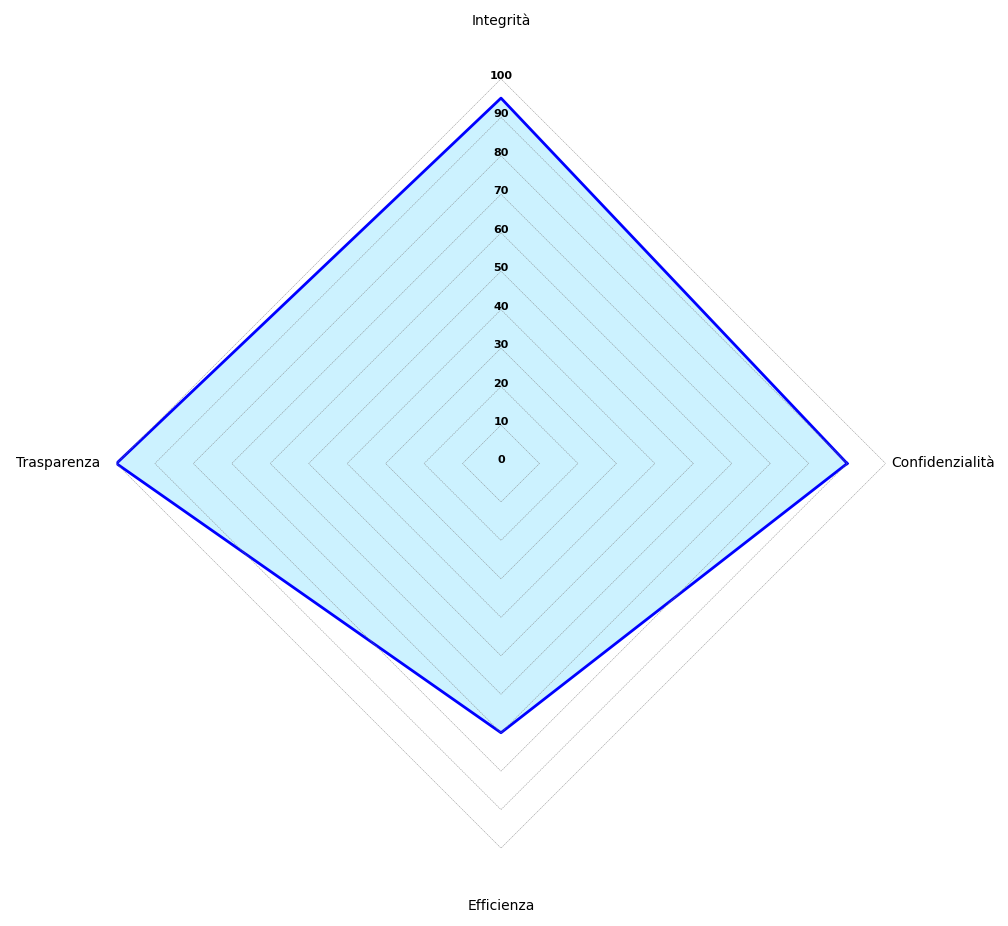
\includegraphics[width=1 \textwidth]{radar.png}
        \caption{Grafico radar relativo alle proprietà}
        \label{radar-graph-properties}
    \end{figure}
    \chapter{WORK PACKAGE 4}
    

\end{document}